\documentclass[11pt,a4paper]{article}
\usepackage{gtu-el-yazisi}
\begin{document}
\notbilgi{Alan Teorisi}{Ders 10 -- Dirac delta fonksiyonu ve yük dağılımları}{Ders10.pdf}

\sayfa{1}
\[
\delta(x-a)=\begin{cases} x\neq a, & 0\\ x=a, & \infty\end{cases}
\]
\noindent
\begin{minipage}[c]{0.34\linewidth}
\centering
\begin{tikzpicture}[line width=0.6pt,murekkep]
  \draw[->] (-1.5,0)--(1.8,0) node[below left]{$x$};
  \draw[->] (0,0)--(0,2.5);
  \fill[pattern=north east lines,pattern color=murekkep] (-1,0) rectangle (1,1);
  \draw (-1,0) rectangle (1,1);
  \draw (-0.45,0) rectangle (0.45,1.9);
  \node[below] at (-1,0) {\small $-\varepsilon$};
  \node[below] at (1,0) {\small $\varepsilon$};
\end{tikzpicture}
\end{minipage}\hfill
\begin{minipage}[c]{0.62\linewidth}
\[
f_\varepsilon(x)=\begin{cases}0; & |x|>\varepsilon\\ 1/2\varepsilon & |x|<\varepsilon\end{cases}
\]
\[
\int_{-\infty}^{\infty}\delta(x-a)\,dx=1
\]
\end{minipage}
\[
S_T=\frac{1}{2\varepsilon}\cdot 2\varepsilon=1\ \Rightarrow\ \lim_{\varepsilon\to 0}S_T=\lim_{\varepsilon\to 0}\frac{1}{2\varepsilon}\,2\varepsilon=\lim_{\varepsilon\to 0}1=1
\]
\[
\delta(x)=\lim_{z\to\infty}\frac{z}{\sqrt\pi}\,e^{-z^2x^2}=\begin{cases}0, & x\neq 0\\ \infty, & x=0\end{cases}
\]
\begin{center}
\begin{tikzpicture}[line width=0.6pt,murekkep]
  \draw[->] (-2.2,0)--(2.4,0);
  \draw (0,-0.3)--(0,1.9);
  \draw[smooth,domain=-2:2,samples=40] plot (\x,{0.9*exp(-(\x*\x)/0.9)});
  \draw[smooth,domain=-2:2,samples=60] plot (\x,{1.3*exp(-(\x*\x)/0.35)});
  \draw[smooth,domain=-2:2,samples=80] plot (\x,{1.7*exp(-(\x*\x)/0.12)});
\end{tikzpicture}
\end{center}
\begin{align*}
\int_{-\infty}^{\infty}\delta(x)\,dx=1&=\int_{-\infty}^{\infty}\lim_{z\to\infty}\frac{z}{\sqrt\pi}\,e^{-z^2x^2}\,dx\\
&=\frac{1}{\sqrt\pi}\lim_{z\to\infty}z\int_{-\infty}^{\infty}e^{-z^2x^2}\,dx
\end{align*}
\[\begin{aligned}
&zx=x'\ \Rightarrow\ dx=\frac{dx'}{z}\\
&\int_{-\infty}^{\infty}\delta_z(x)\,dx=\int_{-\infty}^{\infty}\lim\frac{z}{\sqrt\pi}\,e^{-z^2x^2}\,dx\\
&=\frac{1}{\sqrt\pi}\lim_{z\to\infty}z\int_{x=-\infty}^{\infty}e^{-x'^2}\,\frac{dx'}{z}\\
&=\frac{1}{\sqrt\pi}\lim_{z\to\infty}z\cdot\frac1z\int_{-\infty}^{\infty}e^{-x'^2}\\
&=\frac{1}{\sqrt\pi}\int_{-\infty}^{\infty}e^{-x'}\,dx'=\frac{\sqrt\pi}{\sqrt\pi}=1\quad\text{\footnotemark}
\end{aligned}\footnotetext{Claude notu: üs muhtemelen $-x'^2$ olmalı.}\]
\elcizimi[0.3]{sekiller/Ders10-s1-1.png}[1]

\sayfa{2}
\[
I=\int_{-\infty}^{\infty}e^{-x^2}\,dx=\int_{-\infty}^{\infty}e^{-y^2}\,dy>0
\]
\[
\int_{-\infty}^{\infty}e^{-x^2}\,dx\int_{-\infty}^{\infty}e^{-y}\,dy=I^2\quad\text{\footnotemark}\footnotetext{Claude notu: üs muhtemelen $-y^2$ olmalı.}
\]
\[
I^2=\int_{-\infty}^{\infty}\int_{-\infty}^{\infty}e^{-x^2-y^2}\,dx\,dy
\]
\[
=\int_{-\infty}^{\infty}\int_{-\infty}^{\infty}\underbrace{e^{-(x^2+y^2)}}_{f(x,y)}\,dx\,dy
\]
\elcizimi[0.5]{sekiller/Ders10-s2-1.png}[2]
\begin{align*}
&e^{-(x^2+y^2)}=e^{-\rho^2}\\
&ds=dx\,dy\\
&ds=\rho\,d\phi\,d\rho\\
&0<\rho<\infty\\
&0<\phi<2\pi
\end{align*}
\[
\int_{\rho=0}^{\infty}\int_{\phi=0}^{2\pi}e^{-\rho^2}\,\rho\,d\rho\,d\phi=\frac{2\pi}{-2}\int_{\rho=0}^{\infty}-2\rho\,e^{-\rho^2}\,d\rho
\]
\[
I^2=-\pi\int_{\rho=0}^{\infty}-2\rho\,e^{-\rho^2}\,d\rho=-\pi\,e^{-\rho^2}\Big|_{\rho=0}^{\infty}=-\pi\,(e^{-\infty}-e^{0})=\pi
\]
\[
I=\int_{-\infty}^{\infty}e^{-x^2}\,dx=2\int_0^{\infty}e^{-x^2}\,dx=\sqrt\pi\ \Rightarrow\ \int_0^{\infty}e^{-x^2}\,dx=\frac{\sqrt\pi}{2}
\]

\sayfa{3}
\[
\textcolor{kirmizikalem}{\star}\quad f(x)\,\delta(x-a)=f(a)\,\delta(x-a)
\]
\begin{align*}
\textcolor{kirmizikalem}{\star}\quad\int_{-\infty}^{\infty}f(x)\,\delta(x-a)\,dx&=\int_{-\infty}^{\infty}f(a)\,\delta(x-a)\,dx\\
&=f(a)\int_{-\infty}^{\infty}\delta(x-a)\,dx=f(a)
\end{align*}
\[
\int_{-\infty}^{\infty}\delta(x-a)\,dx=1=\int_{\xi_1}^{\xi_2}\delta(x-a)\,dx=\begin{cases}1, & \xi_1<a<\xi_2\\ 0, & \text{aksi halde}\end{cases}
\]
\noindent
\begin{minipage}[c]{0.70\linewidth}
\[
f(x)=\int_{-\infty}^{x}\delta(z-a)\,dz=\begin{cases}1; & a<x\\ 0; & a>x\end{cases}=u(x)
\]
\end{minipage}\hfill
\begin{minipage}[c]{0.28\linewidth}
\centering
\begin{tikzpicture}[line width=0.6pt]
  \draw[->] (-1.1,0)--(1.4,0);
  \draw[->] (0,-0.1)--(0,1.4);
  \node[left,text=kirmizikalem] at (0,1) {\small $1$};
  \draw[kirmizikalem] (-1.1,0)--(0.5,0)--(0.5,1)--(1.4,1);
\end{tikzpicture}
\end{minipage}
\[
u(x-a)\mathrel{\overset{\scriptscriptstyle\Delta}{=}}\int_{-\infty}^{x}\delta(z-a)\,dz\ \Rightarrow\ \frac{du(x-a)}{d(x-a)}=u'(x-a)=\delta(x-a)
\]
\[
u'(x)\mathrel{\overset{\scriptscriptstyle\Delta}{=}}\delta(x)
\]
\begin{center}
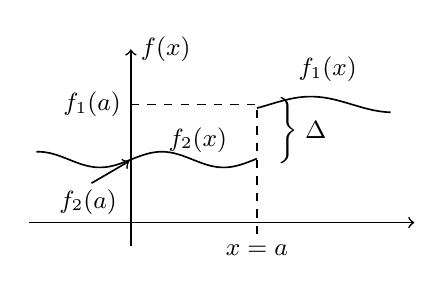
\begin{tikzpicture}[line width=0.6pt]
  \draw[->] (-1.3,0)--(3.6,0);
  \draw[->] (0,-0.3)--(0,2.2) node[right]{\small $f(x)$};
  \draw[smooth] plot[domain=-1.2:1.6,samples=30] (\x,{0.8+0.1*sin((4*\x) r)});
  \draw[smooth] plot[domain=1.6:3.3,samples=30] (\x,{1.5+0.1*sin((3*\x+1) r)});
  \draw[dashed] (1.6,-0.15)--(1.6,1.5);
  \draw[dashed] (0,1.5)--(1.6,1.5);
  \node[left] at (0,1.5) {\small $f_1(a)$};
  \node[below left] at (-0.05,0.55) {\small $f_2(a)$};
  \draw[->] (-0.5,0.5)--(-0.02,0.78);
  \node at (0.85,1.05) {\small $f_2(x)$};
  \node at (2.5,1.95) {\small $f_1(x)$};
  \node at (2.0,1.17) {$\bigg\}$};
  \node at (2.35,1.17) {\small $\Delta$};
  \node[below] at (1.6,-0.15) {\small $x=a$};
\end{tikzpicture}
\end{center}
\[
f(x)=\begin{cases}f_1(x); & x>a\\ f_2(x); & x<a\end{cases}=f_1(x)\,u(x-a)+f_2(x)\,[1-u(x-a)]
\]
\[
f_1(a)-f_2(a)=\Delta
\]
\[\begin{aligned}
f'(x)&=\frac{df(x)}{dx}=\frac{d}{dx}\bigl[f_1(x)\,u(x-a)\bigr]+\frac{d}{dx}\bigl[f_2(x)\,[1-u(x-a)]\bigr]\\
&=f_1'(x)\,u(x-a)+f_1'(x)\,u'(x-a)\text{\footnotemark}+f_2'(x)\,[1-u(x-a)]+f_2(x)\,[1-u(x-a)]'\\
&=f_1'(x)\,u(x-a)+f_2'(x)\,[1-u(x-a)]+f_1(x)\,\delta(x-a)-f_2(x)\,\delta(x-a)\\
&=\begin{cases}f_1'(x); & x>a\\ f_2'(x); & x<a\end{cases}+[f_1(x)-f_2(x)]\,\delta(x-a)\\
&=\begin{cases}f_1'(x); & x>a\\ f_2'(x); & x<a\end{cases}+\underbrace{[f_1(a)-f_2(a)]\,\delta(x-a)}_{\text{tekil kısmı distribüsyondur}}
\end{aligned}\footnotetext{Claude notu: ikinci terim muhtemelen $f_1(x)\,u'(x-a)$ olmalı (çarpım türevi).}\]

\sayfa{4}
\[
V=\begin{cases}V_1(x,y,z); & x>a\\ V_2(x,y,z) & x<a\end{cases}
\]
\[
\Rightarrow\ \mathrm{grad}\,V=\{\mathrm{grad}\,V\}+\vec e_x\,\underbrace{[V_1-V_2]\big|_{x=a}}_{\Delta V|_{x=a}}\,\delta(x-a)
\]
\[
=\begin{cases}\mathrm{grad}\,V_1; & x>a\\ \mathrm{grad}\,V_2; & x<a\end{cases}
\]
\[\begin{aligned}
&=\vec e_x\,(V_1-V_2)\big|_{x=a}\\
&=-\vec e_x\,(V_2-V_1)\big|_{x=a}
\end{aligned}\]
\[
\vec D=\begin{cases}\vec D_1, & x>a\\ \vec D_2, & x<a\end{cases}
\]
\[
\mathrm{div}\,\vec D=\begin{cases}\mathrm{div}\,\vec D_1; & x>a\\ \mathrm{div}\,\vec D_2; & x<a\end{cases}+\vec e_x\,(\vec D_1-\vec D_2)\big|_{x=a}\,\delta(x-a)
\]
\[
\vec n\,\Delta f\big|_S\,\delta(S)
\]
\[
\vec E=\begin{cases}\vec E_1, & x>a\\ \vec E_2, & x<a\end{cases}\ \Rightarrow\ \mathrm{rot}\,\vec E=\left\{\begin{array}{ll}\mathrm{rot}\,\vec E_1; & x>a\\ \mathrm{rot}\,\vec E_2; & x<a\end{array}\right\}
\]
\elcizimi[0.3]{sekiller/Ders10-s4-1.png}[4]
\[
\vec E=-\mathrm{grad}\,V=\begin{cases}\vec E_1\\ \vec E_2\end{cases}+\vec n\,[V_1-V_2]\big|_S\,\delta(S)
\]
\[
\begin{gathered}\downarrow\\ \vec n\,\bigl[V_1\big|_S-V_2\big|_S\bigr]\,\delta(S)\end{gathered}
\]
\[
\vec D_1=\varepsilon_1\vec E_1
\]
\begin{center}
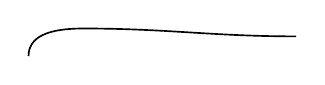
\begin{tikzpicture}[line width=0.6pt]
  \draw (0,0) to[out=90,in=180] (0.7,0.35) to[out=0,in=180] (3.4,0.25);
\end{tikzpicture}
\end{center}
\[
\vec D_2=\varepsilon_2\vec E_2
\]
\[
\vec D=\begin{cases}\vec D_1; & \text{üst}(S)\\ \vec D_2; & \text{alt}(S)\end{cases}
\]
\[
\mathrm{div}\,\vec D=\left\{\begin{array}{ll}\mathrm{div}\,\vec D_1 & \text{üst}(S)\\ \mathrm{div}\,\vec D_2 & \text{alt}(S)\end{array}\right\}+\underbrace{\vec n\,(\vec D_1-\vec D_2)\big|_S}_{\rho_s}\,\delta(S)
\]

\sayfa{5}
\[
\rho=\left\{\begin{array}{l}\rho_1\\ \rho_2\end{array}\right\}+\rho_s\,\delta(S)
\]
\elcizimi[0.35]{sekiller/Ders10-s5-1.png}[5]
\[
\rho=q\,\underbrace{\delta(x-a)}_{1/\mathrm{m}}\,\underbrace{\delta(y-b)}_{1/\mathrm{m}}\,\underbrace{\delta(z-c)}_{1/\mathrm{m}}\quad(\mathrm{C/m^3})
\]
\[
\textcolor{kirmizikalem}{\rho=\frac{dq}{dv}=\infty}
\]
\elcizimi[0.4]{sekiller/Ders10-s5-2.png}[5]
\[
\rho=\rho_s\,\delta(x-a)\,\delta(y-b)\quad\text{\footnotemark}\footnotetext{Claude notu: sonsuz doğru yükü için çizimdeki $\rho_c$ (C/m) beklenir; $\rho_s$ yüzey yük yoğunluğudur.}
\]
\elcizimi[0.3]{sekiller/Ders10-s5-3.png}[5]
\[
\rho=\rho_s\,\delta(z-a)\quad(\mathrm{C/m^3})
\]

\sayfa{6}
\elcizimi[0.4]{sekiller/Ders10-s6-1.png}[6]
\[\begin{aligned}
\rho&=\rho_c\,\delta(x-a)\,\delta(y-b)\,\bigl[u(z-z_1)+u(z-z_2)\bigr]\quad\text{\footnotemark}\\
&=\rho_c\,\delta(x-a)\,\delta(y-b)\qquad z_2<z<z_1
\end{aligned}\footnotetext{Claude notu: $z_2<z<z_1$ için muhtemelen $\bigl[u(z-z_2)-u(z-z_1)\bigr]$ olmalı.}\]
\[\begin{aligned}
\sin x\,\delta(x)&=\sin 0\,\delta(x)=0\\
\cos x\,\delta(x)&=\cos\,\delta(x)=\delta(x)\quad\text{\footnotemark}\\
\tan(x)\,\delta(x-\pi)&\\
&=\tan(\pi)\,\delta(x-\pi)=0\quad/\!/
\end{aligned}\footnotetext{Claude notu: $\cos 0$ olmalı.}\]
\elcizimi[0.3]{sekiller/Ders10-s6-2.png}[6]
\[
\rho=\rho_s\,\delta(z-a)\,\bigl[u(y-y_1)-u(y-y_2)\bigr]\bigl[u(x-x_2)-u(x-x_1)\bigr]
\]
\[
y\ \okunamadi{<}\ y_1<y_2
\]
\end{document}
